\documentclass[12pt,a4paper,oneside]{article}
\usepackage[utf8]{inputenc}
\usepackage{amsmath}
\usepackage{amsfonts}
\usepackage{amssymb}
\usepackage{fancyhdr}
\usepackage{bigints}
\usepackage{mathrsfs}
\usepackage{subfigure}
\usepackage{subfig}
\usepackage{float}
\usepackage{listings}
\usepackage{multicol}
\usepackage{makeidx}
\usepackage{subcaption}
\usepackage{caption}
\usepackage{lipsum}
\usepackage{graphicx}
\usepackage[export]{adjustbox}
\usepackage[dvipsnames]{xcolor}
\definecolor{blue-violet}{rgb}{0.54, 0.17, 0.89}
\usepackage{xcolor}
\usepackage{setspace}
\usepackage{draftwatermark}
\SetWatermarkText{Neutrosophic Extension of Weibull Distribution in Reliability Model}
\SetWatermarkScale{1}
\usepackage[left=2.3cm,right=1.5cm,top=2cm,bottom=2cm]{geometry}
\usepackage{blindtext}
\usepackage{background}
\usetikzlibrary{calc}
\backgroundsetup{angle = 0, scale = 1, vshift = -2ex,
  contents = {\tikz[overlay, remember picture]
    \draw [rounded corners = 20pt, line width = 1pt,
           color = black, fill = white!20, double = black!10]
           ($(current page.north west)+(1.5cm,-1cm)$)
           rectangle ($(current page.south east)+(-0.1,1)$);}}
\pagestyle{empty}
\pagenumbering{arabic}
\author{Saunak Mitra}
\begin{document}
\vspace*{3cm}
\begin{singlespace}
\begin{Large}
\hspace*{6cm}\textrm{\textit{\textbf{\underline{Abstract}}}}
\end{Large}
\end{singlespace}
\vspace*{1cm}
The Neutrosophic Weibull Distribution (NWD) is a versatile probabilistic model that integrates the Neutrosophic Set Theory with the Weibull distribution. It provides a robust framework for handling uncertainty in real-world data, particularly in scenarios where traditional statistical methods may fall short. The (NWD) captures the imprecise, indeterminate, and contradictory aspects of data, offering a more comprehensive representation of uncertainty. This abstract explores the theoretical foundation, statistical properties, and potential applications of the proposed distribution.Weibull Distribution is widely used for Reliability/survival analysis.But in most of the real life cases it is impossible to identify and precisely account of all factors.To,deal with this we move to neutrosophic approach.Though the neutrosophic weibull distribution model was proposed before by "Kawther Fawzi Hamza Alhasan and Florentin Smarandache" but here we derive all the theoritical derivations thoroughly and the simulate the data from the mentioned distribution and the approach of maximum likelihood estimation is applied to estimate the parameters and using those estimated values we validate our model based on the evaluated performance of the proposed model.
\newpage
\begin{singlespace}
\begin{Large}
\textrm{\textit{\textbf{\underline{Introduction:$-$}}}}
\end{Large}
\end{singlespace}
\vspace*{5mm}
The Neutrosophic Extension of the Weibull Distribution represents a significant advancement in reliability modeling, offering a nuanced approach to capturing uncertainties inherent in complex systems. Reliability analysis plays a pivotal role in various fields such as engineering, healthcare, and finance, where understanding and predicting the lifetimes of systems or components is critical for decision-making and risk management.\\

The traditional Weibull distribution has long been a cornerstone in reliability engineering due to its flexibility in modeling failure rates over time. However, conventional statistical methods often struggle to account for the inherent ambiguity and vagueness present in real-world data, especially in scenarios where information is incomplete or imprecise.\\

The Neutrosophic Extension of the Weibull Distribution addresses this challenge by integrating the principles of neutrosophic set theory into the reliability modeling framework. Neutrosophy, introduced by Florentin Smarandache, extends the concepts of classical set theory to accommodate indeterminacy, ambiguity, and contradictions through the notion of truth-membership, indeterminacy-membership, and falsehood-membership degrees.\\

In the context of reliability modeling, neutrosophic set theory enables us to represent and quantify uncertainties that arise from various sources such as measurement errors, subjective judgments, or incomplete information. By allowing for the characterization of vague or incomplete data, the neutrosophic extension enriches the descriptive power of the Weibull distribution, making it more adaptable to real-world scenarios where precise probabilistic modeling may be inadequate.\\

The incorporation of neutrosophic elements into the Weibull distribution empowers analysts to more accurately model and analyze complex systems' failure patterns, particularly in situations where traditional statistical approaches may fall short. Moreover, this extension opens avenues for exploring new dimensions of uncertainty and variability, leading to more robust and insightful reliability assessments.\\

In summary, the Neutrosophic Extension of the Weibull Distribution represents a promising frontier in reliability modeling, offering a principled framework for grappling with the inherent uncertainties and ambiguities present in real-world data. As researchers continue to explore and refine this approach, its potential applications across diverse domains are likely to expand, fostering deeper insights into the dynamics of complex systems and enhancing decision-making processes.
\newpage
\textrm{\textit{\textbf{\underline{Weibull Distribution in Reliability Model:$-$}}}}\\
Weibull distribution is a very renowned distribution used in reliability.For example, we can consider the lifetime of a human follows this type of distribution.Where in the first part we can observe a decreasing hazard rate because when a new baby born they has a higher chance of failure and slowly the risk decreases.After a certain age the risk of failure becomes stable.so a constant hazard  rate can be observed.and after age $60$ again the chance of failure increases.So,now we can observe a increasing hazard rate.So,a bathtub type of hazard curve which follows Weibull distribution can be seen.The bathtub curve can be observed if we consider a mixture model of two weibull distribution one having shape parameter $<1$ and the other one having shape parameter $>1$. \\
\newline
\begin{center}
\hspace{2cm}
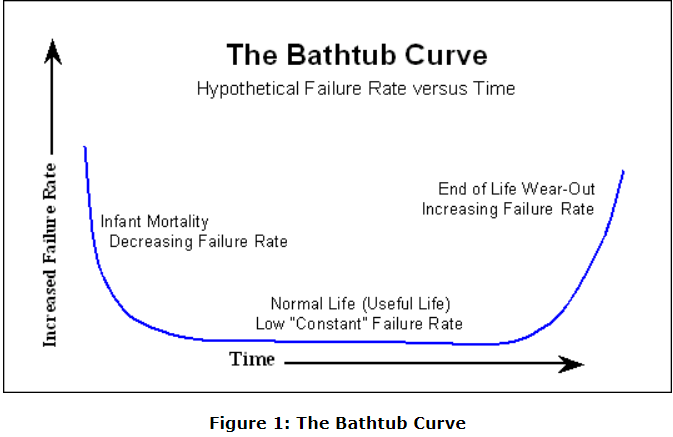
\includegraphics[width=0.7\textwidth]{bathtub}
\newline 
\end{center}
\vspace{2cm}
\textrm{\textit{\textbf{\underline{Weibull Distribution and it's characteristics:$-$}}}}\\
\newline
The pdf of weibull distribution is given by,\\
\newline
\begin{singlespace}
\hspace{5cm}$f_{X}$(x;${\lambda}$,k)=$\dfrac{k}{{\lambda}}$ $\left(\dfrac{x}{\lambda}\right)^{k-1}$ $e^{-\left(\dfrac{x}{\lambda}\right)^{k}}$ \hspace{1cm}, $x \geq 0$\\
\end{singlespace}
\hspace{6.7cm}=0 \hspace{4.1cm} ,$x < 0$\\
\newline\newline
So the cdf of weibull distribution will be,\\
\begin{singlespace}
\hspace{5cm}$F_{X}$(x;${\lambda}$,k)=$ \int_{0}^{x}$ $f_{T}$(t;${\lambda}$,k)dt \hspace{1cm}, $x \geq 0$\\
\end{singlespace}
\hspace{6.7cm}=0 \hspace{3.3cm} ,$x < 0$\\
\newpage which implies,
\begin{singlespace}
\hspace{5cm}$F_{X}$(x;${\lambda}$,k)=$ \bigint_{0}^{x}$ $\dfrac{k}{{\lambda}}$ $\left(\dfrac{t}{\lambda}\right)^{k-1}$ $e^{-\left(\dfrac{t}{\lambda}\right)^{k}}$dt
\end{singlespace}
Substituting $\left(\dfrac{t}{\lambda}\right)^{k}$ = p we get,
\begin{singlespace}
\hspace{5cm}$F_{X}$(x;${\lambda}$,k)=$ \bigint_{0}^{\left(\dfrac{x}{\lambda}\right)^{k}}$ $e^{-p}$dp
\end{singlespace}\vspace{2cm}
which simplifies to,
\begin{singlespace}
\hspace{5cm}$F_{X}$(x;${\lambda}$,k)=1$-e^{-\left(\dfrac{x}{\lambda}\right)^{k}}$ \hspace{1cm}, $x \geq 0$\\
\end{singlespace}
\hspace{6.7cm}=0 \hspace{2.7cm} ,$x < 0$\\
\newline\newline
The graph of Weibull distribution depends on it's parameter,it looks like\\
\newline\newline
\begin{center}
\hspace{2cm}
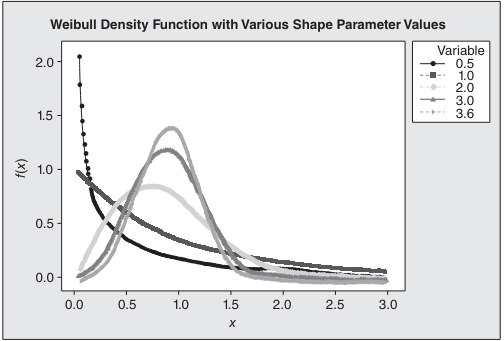
\includegraphics[width=0.7\textwidth]{pdf}
\newline 
Figure 2: Weibull pdf for various values of the shape parameter k
\end{center}
\begin{center}
\hspace{2cm}
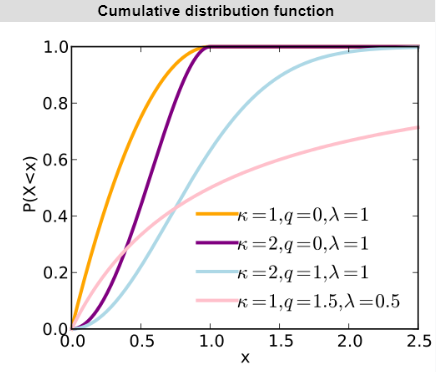
\includegraphics[width=0.7\textwidth]{cdf}
\newline 
Figure 3: Weibull cdf for various values of the parameters
\end{center}
\vspace{2cm}
So, the Reliability function is given by,\\
$\omega_{X}(x;{\lambda}$,k)=1-$F_{X}$(x;${\lambda}$,k)=$e^{-\left(\dfrac{x}{\lambda}\right)^{k}}$\newline\newline\newline
The hazard function of Weibull dsitribution is given by,\
h(x;${\lambda}$,k)=$\dfrac{f_{X}(x;{\lambda},k)}{\omega_{X}(x;{\lambda},k)}$=$\dfrac{k}{{\lambda}}$ $\left(\dfrac{x}{\lambda}\right)^{k-1}$
\newline\newline\newline The expectation of Weibull distribution is defined as,\\
\begin{center}
\hspace{5cm}E(x)=$\bigint_{0}^{\infty}$ $xf_{X}$(x;${\lambda}$,k)dx\newline\newline
\begin{singlespace}
\hspace{5.5cm}=$\bigint_{0}^{\infty}$ $x\left(\dfrac{k}{{\lambda}}\right)$ $\left(\dfrac{x}{\lambda}\right)^{k-1}$ $e^{-\left(\dfrac{x}{\lambda}\right)^{k}}$dx
\end{singlespace}
\end{center}\newpage
substituting $\left(\dfrac{x}{{\lambda}}\right)^{k}$=t we get,\\
\newline
\hspace{2cm}$\left(\dfrac{k}{\lambda}\right)\left(\dfrac{x}{{\lambda}}\right)^{k-1}$dx=dt\\
\newline so it simplifies to,
\begin{center}
\hspace{3cm}E(x)=${\lambda}$ $\bigint_{0}^{\infty}$ $t^{\dfrac{1}{k}+1-1}e^{-t}$dt\\
\begin{singlespace}
\hspace{2cm}$=\boxed{{\lambda}\Gamma\left(\dfrac{1}{k}+1\right)}$
\end{singlespace}
\end{center}
\vspace{2cm}the second order raw moment of order two of weibull distribution is,\\
\begin{center}
\hspace{5cm}E($x^{2}$)=$\bigint_{0}^{\infty}$ $x^{2}f_{X}$(x;${\lambda}$,k)dx\newline\newline
\begin{singlespace}
\hspace{5.7cm}=$\bigint_{0}^{\infty}$ $x^{2}\left(\dfrac{k}{{\lambda}}\right)$ $\left(\dfrac{x}{\lambda}\right)^{k-1}$ $e^{-\left(\dfrac{x}{\lambda}\right)^{k}}$dx
\end{singlespace}
\end{center}
substituting $\left(\dfrac{x}{{\lambda}}\right)^{k}$=t we get,\\
\newline
\hspace{2cm}$\left(\dfrac{k}{\lambda}\right)\left(\dfrac{x}{{\lambda}}\right)^{k-1}$dx=dt\\
\newline so it simplifies to,
\begin{center}
\hspace{3cm}E($x^{2}$)=${\lambda}^{2}$ $\bigint_{0}^{\infty}$ $t^{\dfrac{2}{k}+1-1}e^{-t}$dt\\
\begin{singlespace}
\hspace{3.2cm}$=\boxed{{\lambda}^{2}\Gamma\left(\dfrac{2}{k}+1\right)}$
\end{singlespace}
\end{center}
So the form of variance will  be written as,\\
\newline
var(X)=E($x^{2})-(E(x))^{2}$\\
\newline
i.e, var(X)$=\boxed{{\lambda}^{2}\Gamma\left(\dfrac{2}{k}+1\right)$ $-$ $\left({\lambda}\Gamma\left(\dfrac{1}{k}+1\right)\right)^{2}}$\\
\newline
Similarly,third order raw moment E($x^{3}$)is equal to  ${\lambda}^{3}\Gamma\left(\dfrac{3}{k}+1\right)$\\
\newline\newline So,the third order central moment can be denoted as,$\mu_{3}$=E($x^{3}$) $-$ 3E(x)E($x^{2}$) $+2E(x)^{3}$\\
\newline\newline So,$\mu_{3}$=$\boxed{{\lambda}^{3}\Gamma\left(\dfrac{3}{k}+1\right)$ $-$ 3${\lambda}^{3}\Gamma\left(\dfrac{1}{k}+1\right)$ $\Gamma\left(\dfrac{2}{k}+1\right)$ $+$2${\lambda}^{3}\Gamma\left(\dfrac{1}{k}+1\right)^{3}}$\\
\newpage So, the measure of skewness will be,\\$\boxed{S_{k}$=$\dfrac{\mu_{3}}{\mu_{2}^{\dfrac{3}{2}}}=\left(\dfrac{\Gamma\left(\dfrac{3}{k}+1\right) - 3\Gamma\left(\dfrac{1}{k}+1\right) \Gamma\left(\dfrac{2}{k}+1\right) +2\Gamma\left(\dfrac{1}{k}+1\right)^{3}}{\left(\Gamma\left(\dfrac{2}{k}+1\right) - \left(\Gamma\left(\dfrac{1}{k}+1\right)\right)^{2}\right)^{\dfrac{3}{2}}}\right)}$\\
\newline\newline
Depending on the values of the parameters we can infer if the distribution is positively skewed,negetively skewed or almost symmetric.
Kurtosis is defined as,\\
\newline\newline $\boxed{\dfrac{\mu_{4}}{\mu_{2}^{2}}$=$\left(\dfrac{\Gamma\left(\dfrac{4}{k}+1\right)-4\Gamma\left(\dfrac{3}{k}+1\right)\Gamma\left(\dfrac{1}{k}+1\right)+6\Gamma\left(\dfrac{2}{k}+1\right)\left(\Gamma\left(\dfrac{1}{k}+1\right)\right)^{2}-3\left(\Gamma\left(\dfrac{1}{k}+1\right)\right)^{4}}{\left(\Gamma\left(\dfrac{2}{k}+1\right)-\left(\Gamma\left(\dfrac{1}{k}+1\right)\right)^{2}\right)^{2}}\right)}$\\
\newline\newline Weibull distribution can be leptokurtic,mesokurtic,platykurtic vased on it's shape parameter k. if k$>$2  then the distribution can be leptokurtic.
\newpage
\textrm{\textit{\textbf{\underline{What is meant by Neutrsophic ?$-$}}}}\\
Neutrosophy, introduced by Florentin Smarandache in the late 20th century, is a philosophical concept that deals with indeterminacy, contradiction, and incomplete information. Neutrosophy recognizes that in many real-world scenarios, elements can possess not only true and false values but also indeterminate values lying between true and false. This concept of indeterminacy is crucial in understanding the complexities of human perception and cognition.Neutrosophic logic, an extension of classical and fuzzy logic, provides a framework to handle indeterminacy by introducing the notion of neutrosophic set theory. In a neutrosophic set, elements can belong not only to the set (true), its complement (false), or both, but also to the indeterminate set (neither true nor false). This allows for a more nuanced representation of uncertainty in data and knowledge.Neutrosophic statistics, therefore, applies neutrosophic logic to statistical analysis, enabling the handling of uncertain, imprecise, or incomplete information in data. It extends traditional statistical methods to accommodate situations where classical approaches may fall short due to the presence of ambiguity or contradictory evidence. Neutrosophic statistics finds applications in various domains such as decision-making, pattern recognition, image processing, and artificial intelligence, where dealing with uncertainty is essential for making informed decisions and drawing meaningful conclusions from data.\newline\newline
\textrm{\textit{\textbf{\underline{Neutrosophic  Sets :-$-$}}}}\\
Neutrosophic sets, an extension of classical and fuzzy sets, incorporate the notion of indeterminacy. In a neutrosophic set, elements can belong not only to the set (true) or its complement (false), but also to an indeterminate subset (neither true nor false). This accommodates situations where the truth value of an element is uncertain, vague, or contradictory. Neutrosophic sets provide a framework for representing and reasoning with incomplete or imprecise information, allowing for a more flexible and nuanced approach to modeling uncertainty in various fields such as decision making, pattern recognition, and artificial intelligence.\newline\newline
\textrm{\textit{\textbf{\underline{Neutrosophic probability :- $-$}}}}\\
Neutrosophic probability is a theory that extends classical probability theory to handle uncertainty in a more nuanced manner. It deals with situations where the probabilities of events are uncertain, imprecise, or indeterminate. Unlike classical probability, which assigns precise probabilities to events, neutrosophic probability allows for the representation of indeterminacy, ambiguity, and contradiction in probability assessments. It introduces the notion of neutrosophic events, where the likelihood of occurrence lies within a range of values rather than a single probability. Neutrosophic probability finds applications in decision making, risk analysis, and other domains where dealing with uncertain or incomplete information is essential.\\The function that models the neutrosophic probability of a random variable x is called neutrosophic distribution:NP(x)= (T(x), I(X), F(x) ) , where  T(x) represents the probability that the value x occurs , F(x) represents the probability that the value x does not occurs,and I(X) represents the indeterminate $/$ unknown probability of value x to occur or not.\newline\newline
\textrm{\textit{\textbf{\underline{Neutrosophic statistics :- :- $-$}}}}\\
Neutrosophic statistics is a statistical framework that extends traditional statistics to handle uncertainty, ambiguity, and indeterminacy in data analysis. It incorporates neutrosophic logic to accommodate situations where data may be vague or incomplete, allowing for a more comprehensive treatment of uncertainty. Neutrosophic statistics provides methods for analyzing and interpreting data sets that contain imprecise or contradictory information, enabling researchers and practitioners to make informed decisions in the presence of uncertainty. This approach finds applications in various fields such as decision making, pattern recognition, and machine learning, where dealing with uncertain or incomplete data is common.
\newpage
 \textrm{\textit{\textbf{\underline{Weibull Distribution in Neutrosophic approach:$-$}}}}\\
 In neutrosophic distribution we proceed as same as classical way but the moments such as mean and the parameters are not proper or imprecise.Neutrosophic concept actually gives idea about indeterminancy value present in real world.\\
 \newline In neutrosophic context, the pdf of Weibull distribution is defined as,\\
 \hspace{5cm}$f_{X}$(x;${\lambda},k_{N}$)=$\dfrac{k_{N}}{\lambda_{N}}$ $\left(\dfrac{x}{\lambda_{N}}\right)^{k_{N}-1}$ $e^{-\left(\dfrac{x}{\lambda_{N}}\right)^{k_{N}}}$ \hspace{1cm}, $x \geq 0$\\
 \newline \newline where $k_{N}=[k_{l},k_{u}]$ and $\lambda_{N}=[\lambda_{l},\lambda_{u}]$\\
 \newline In classical model we use $k_{l}=k_{u}=k$ and $\lambda_{l}=\lambda_{u}=\lambda$ and if we take $k_{N}$=[1,1] then the distribution becomes neutrosophic exponential model.\\
 \newline\newline The cumulative distribution distribution function is jointly coupled form of df is given by,\\
 \begin{singlespace}
\hspace{5cm}$F_{N}$(x;${\lambda_{N}},k_{N})=1-e^{-\left(\dfrac{x}{\lambda_{N}}\right)^{k_{N}}}$ \hspace{1cm}, $x \geq 0$\\
\end{singlespace}
\vspace*{3mm} The survival function or reliability function is defined as,\\
\begin{singlespace}
\hspace{5cm}$S_{N}$(x;${\lambda_{N}},k_{N})=1-F_{N}$(x;${\lambda_{N}},k_{N})=e^{-\left(\dfrac{x}{\lambda_{N}}\right)^{k_{N}}}$ 
\end{singlespace}
Hazard function of neutrosophic weibull distribution is defined as,\\
\begin{singlespace}
\hspace{5cm}$h_{N}(x;{\lambda_{N}},k_{N})=\dfrac{f_{N}(x;{\lambda_{N}},k_{N})}{S_{N}(x;{\lambda_{N}},k_{N})}=\dfrac{k_{N}}{\lambda_{N}}$ $\left(\dfrac{x}{\lambda_{N}}\right)^{k_{N}-1}$
\end{singlespace}
\vspace*{2mm}various values of our neutrosophic scale and shape parameters gives us different graphs.\\So, we consider 4 sets of values for which we observe the density curve and the cdf curve and the survival function curve as given below,
 \newpage
\begin{figure}
\centering  
\subfigure[$k_{N}=(0.3,0.5)$]{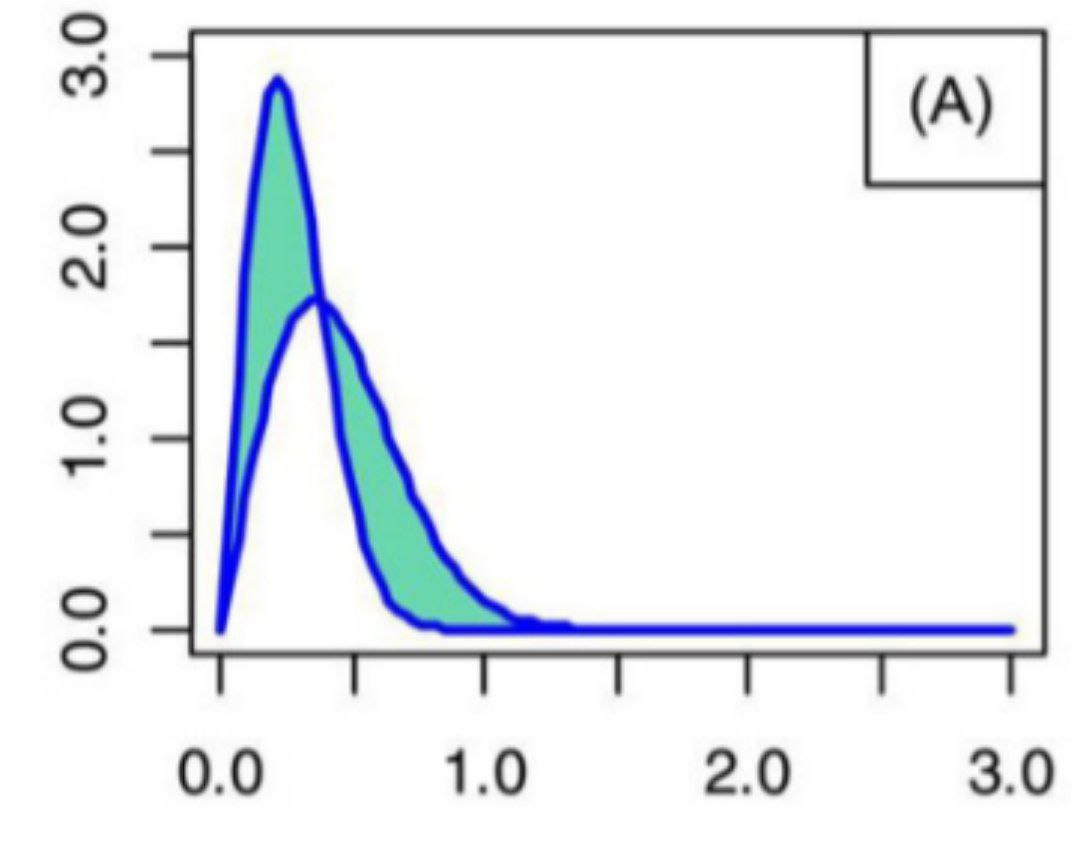
\includegraphics[width=0.35\linewidth]{photo1}}
\subfigure[$k_{N}$=(0.5,1)]{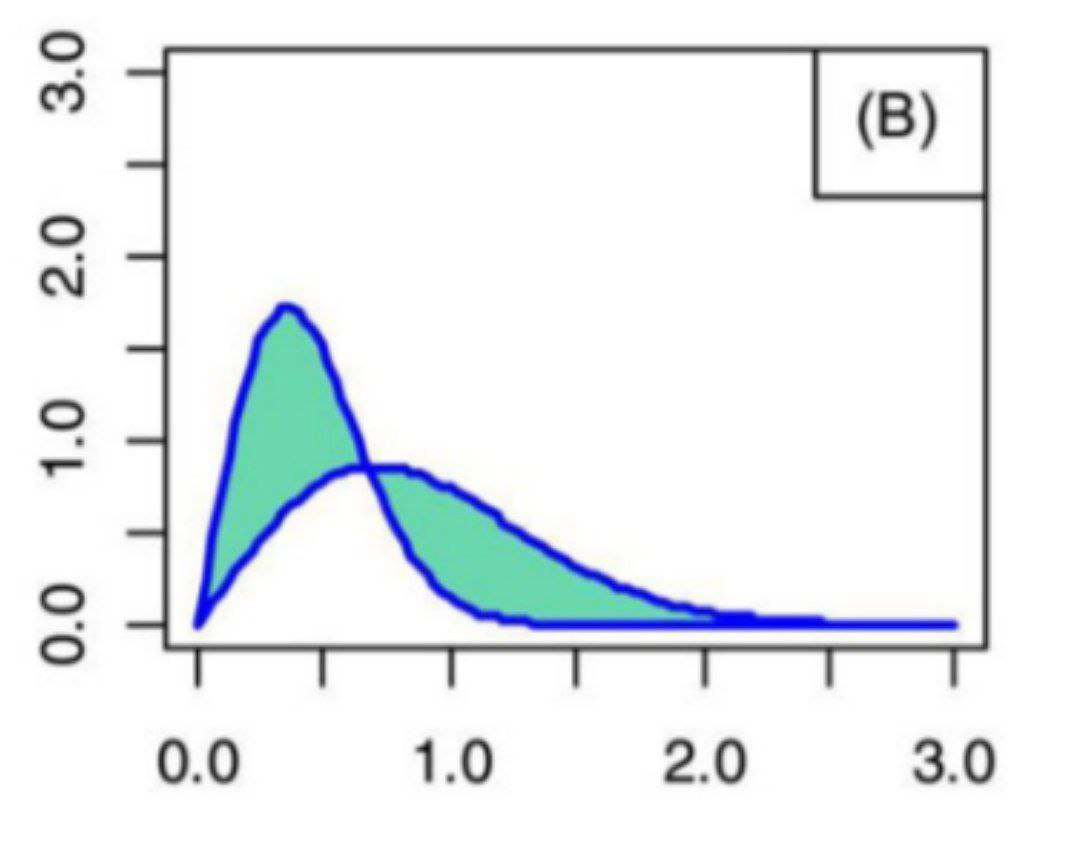
\includegraphics[width=0.35\linewidth]{photo2}}
\subfigure[$k_{N}$=(1.5,2)]{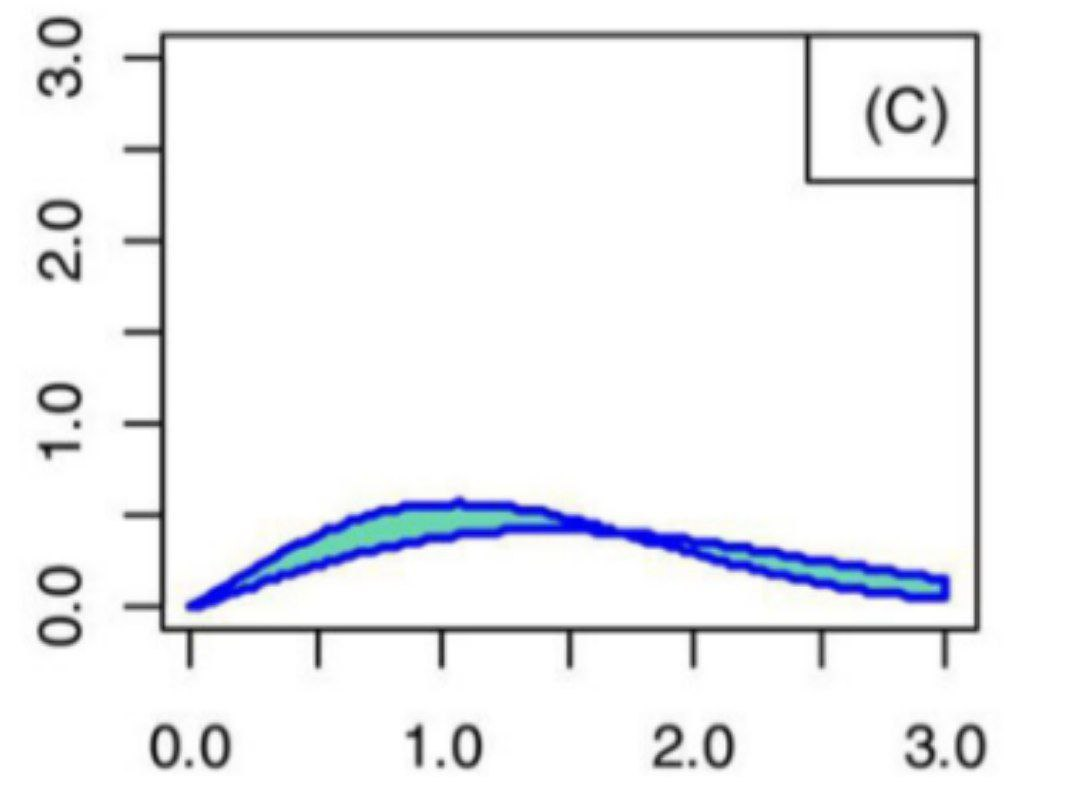
\includegraphics[width=0.35\linewidth]{photo3}}
\subfigure[$k_{N}$=(2,2.5)]{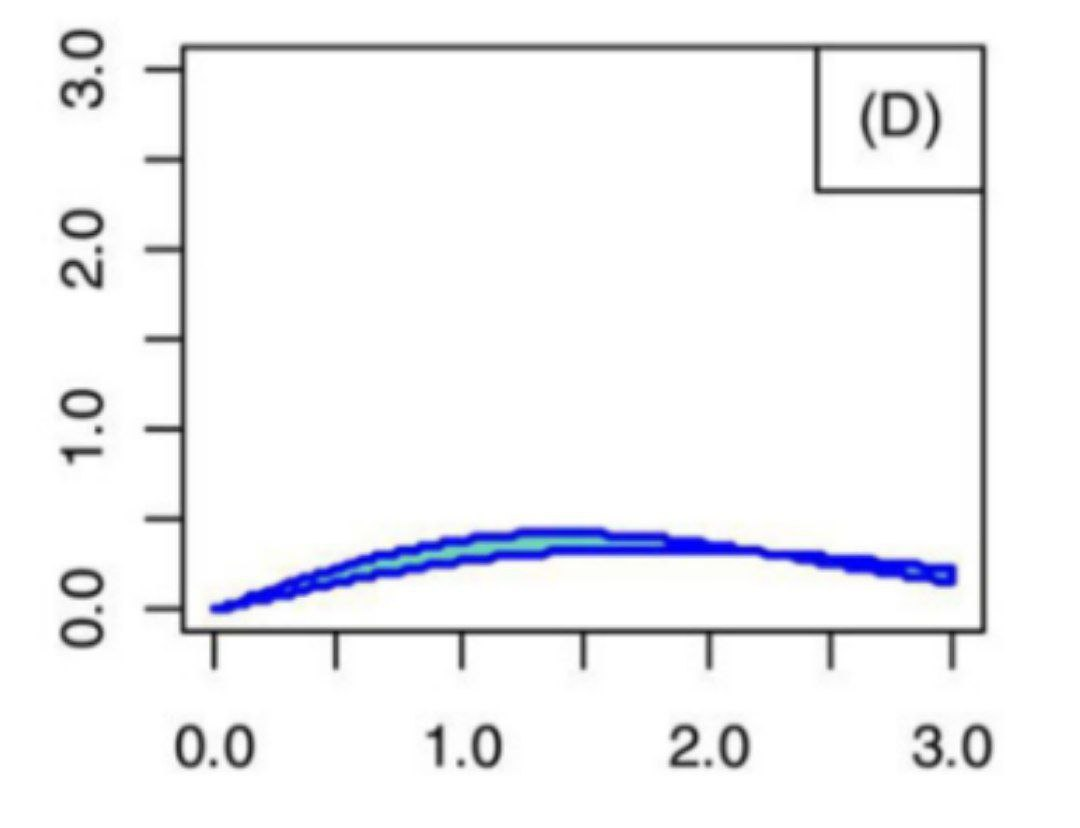
\includegraphics[width=0.35\linewidth]{photo4}}
\caption{ pdf of neutrosophic weibull distribution with different shape parameters}
\end{figure}
\begin{figure}
\centering  
\subfigure[$k_{N}$=(0.3,0.5)]{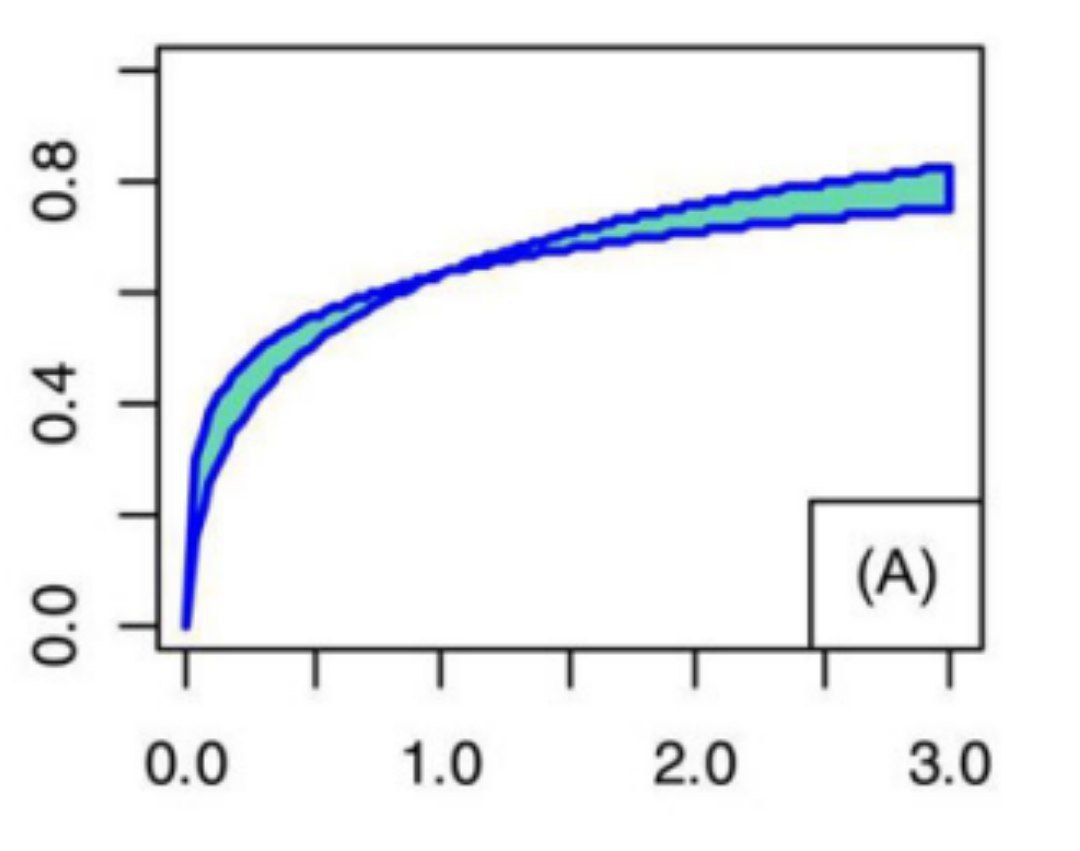
\includegraphics[width=0.35\linewidth]{a}}
\subfigure[$k_{N}$=(0.5,1)]{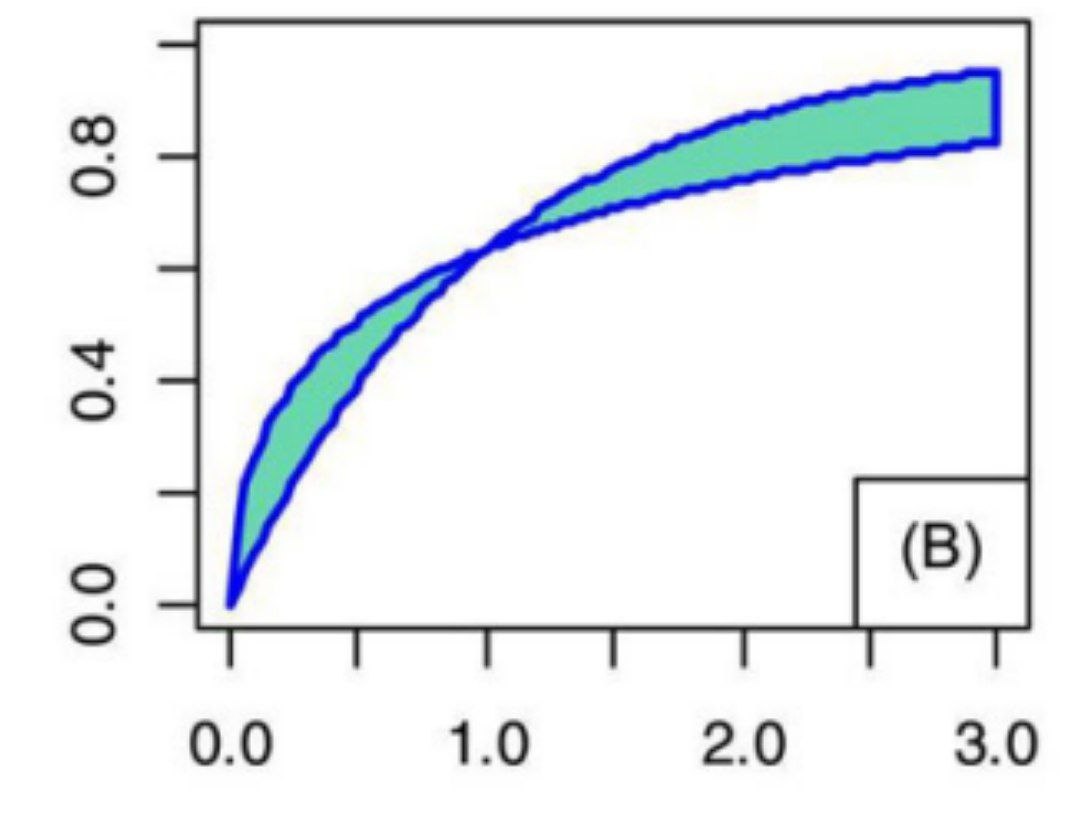
\includegraphics[width=0.35\linewidth]{b}}
\subfigure[$k_{N}$=(1.5,2)]{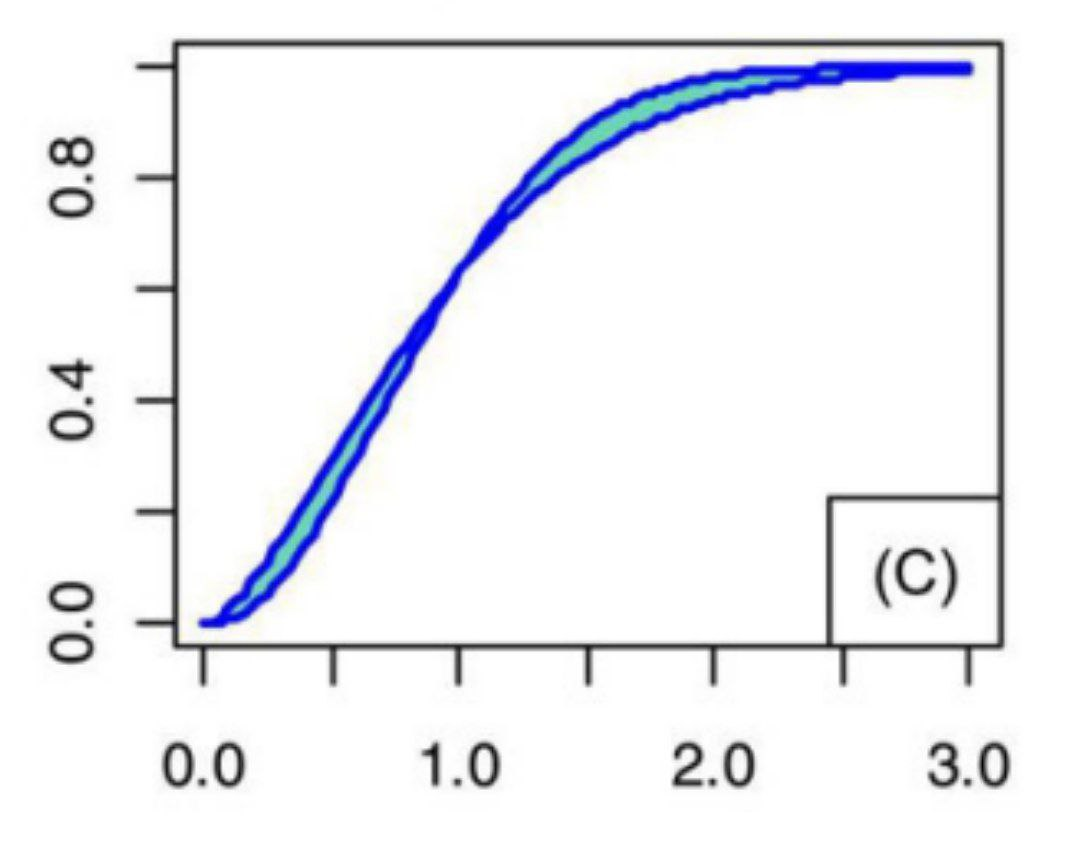
\includegraphics[width=0.35\linewidth]{c}}
\subfigure[$k_{N}$=(2,2.5)]{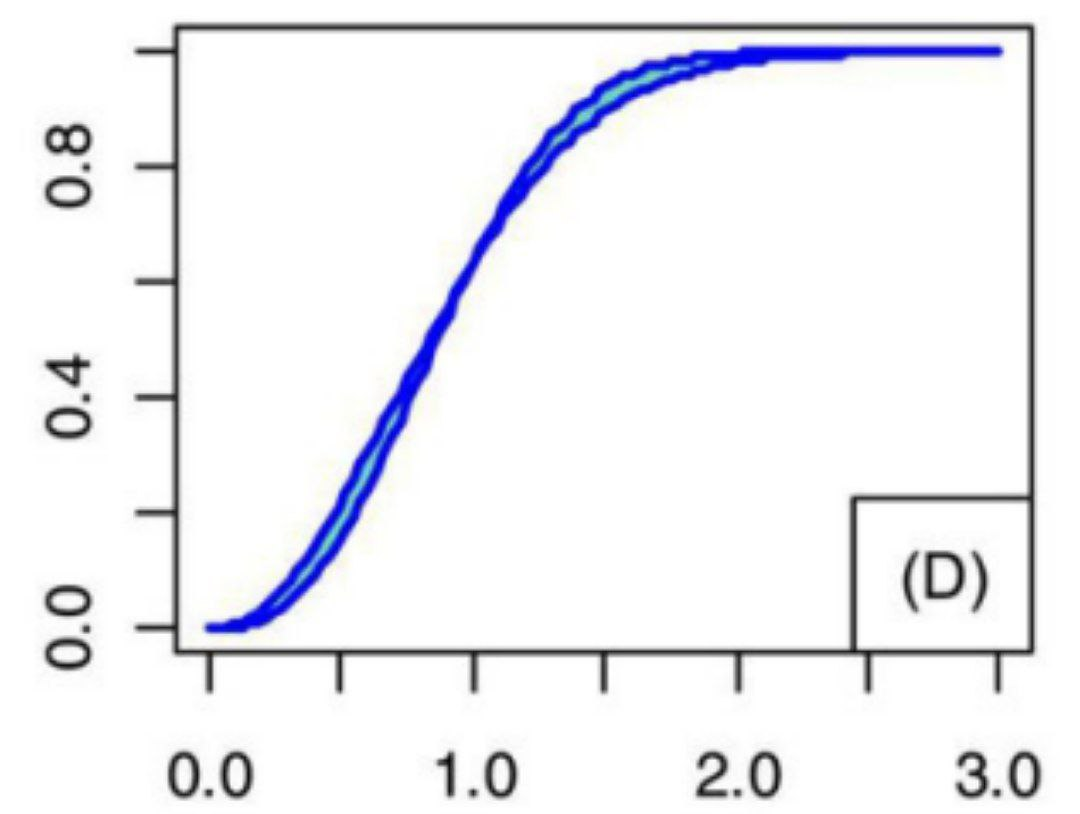
\includegraphics[width=0.35\linewidth]{d}}
\caption{ cdf of neutrosophic weibull distribution with different shape parameters}
\end{figure}
\begin{figure}
\centering  
\subfigure[$k_{N}$=(0.3,0.5)]{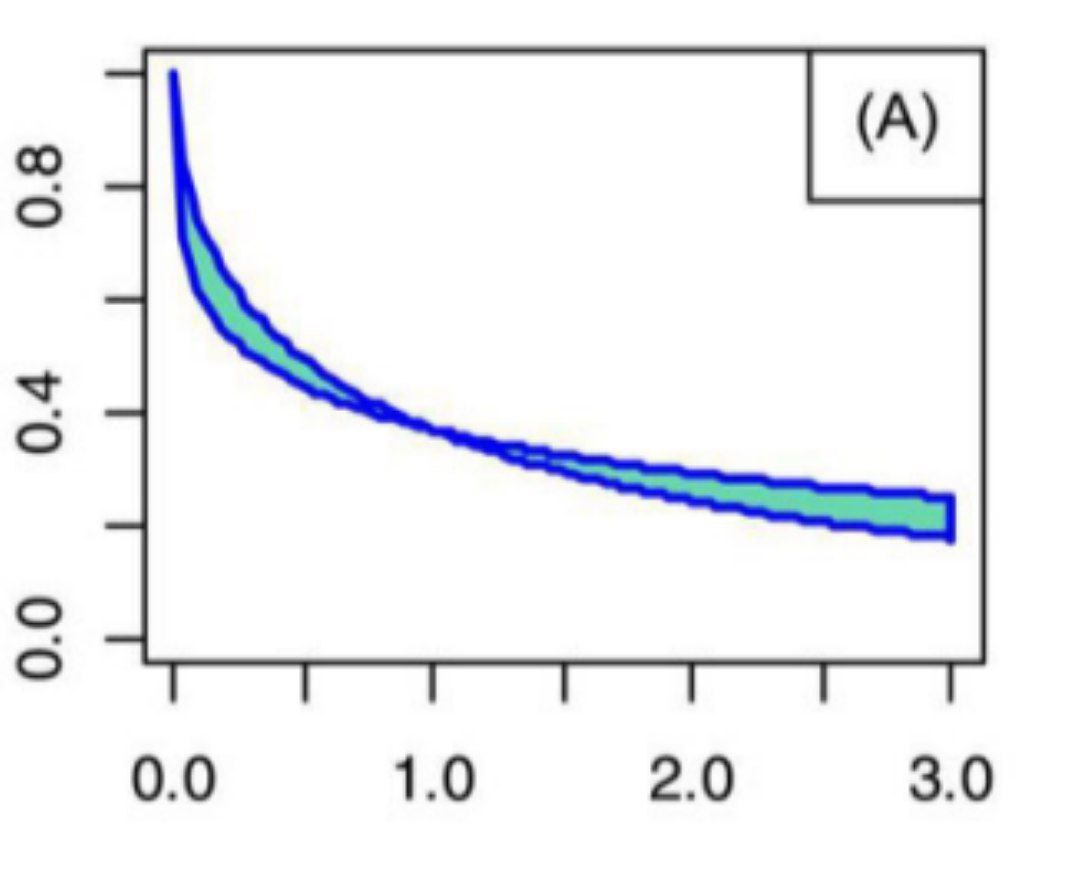
\includegraphics[width=0.35\linewidth]{e}}
\subfigure[$k_{N}$=(0.5,1)]{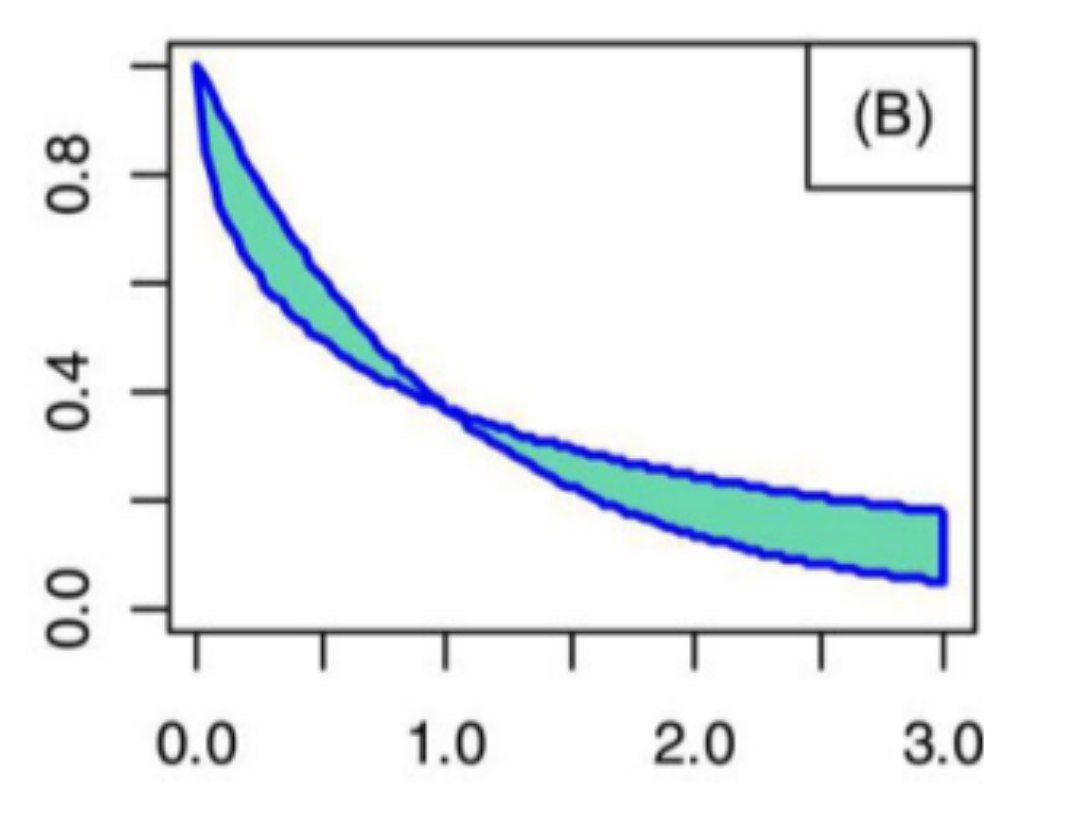
\includegraphics[width=0.35\linewidth]{f}}
\subfigure[$k_{N}$=(1.5,2)]{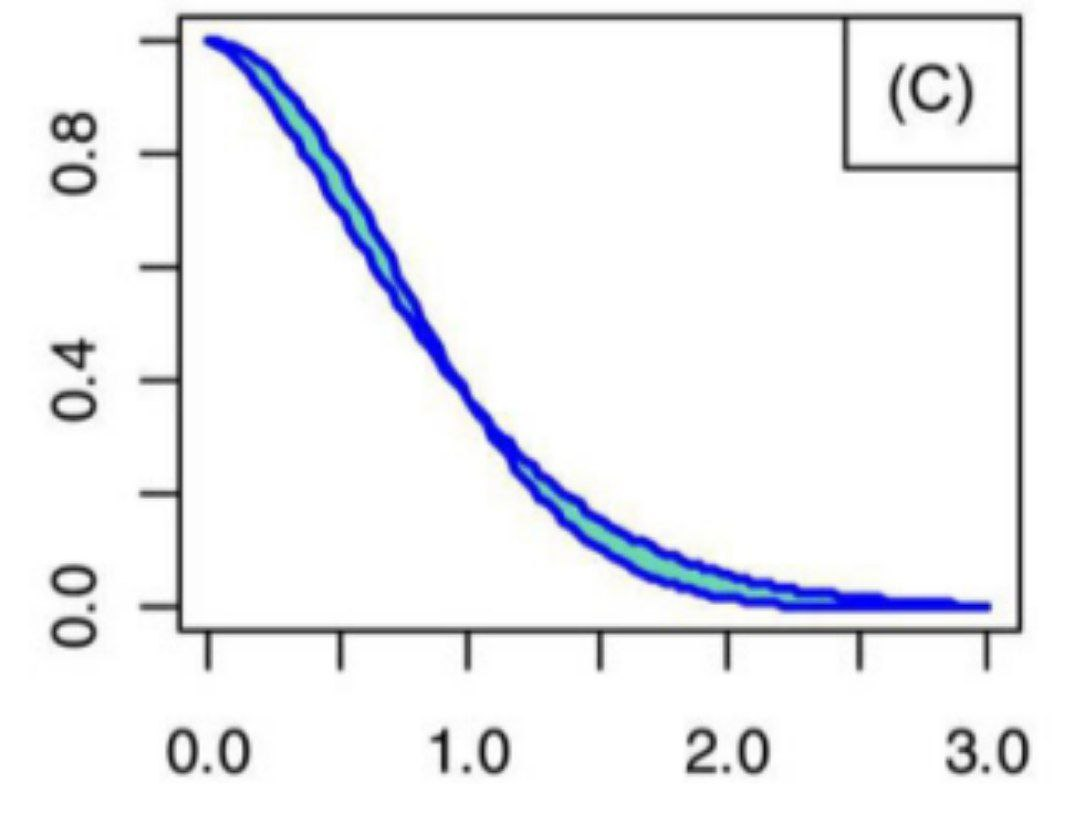
\includegraphics[width=0.35\linewidth]{g}}
\subfigure[$k_{N}$=(2,2.5)]{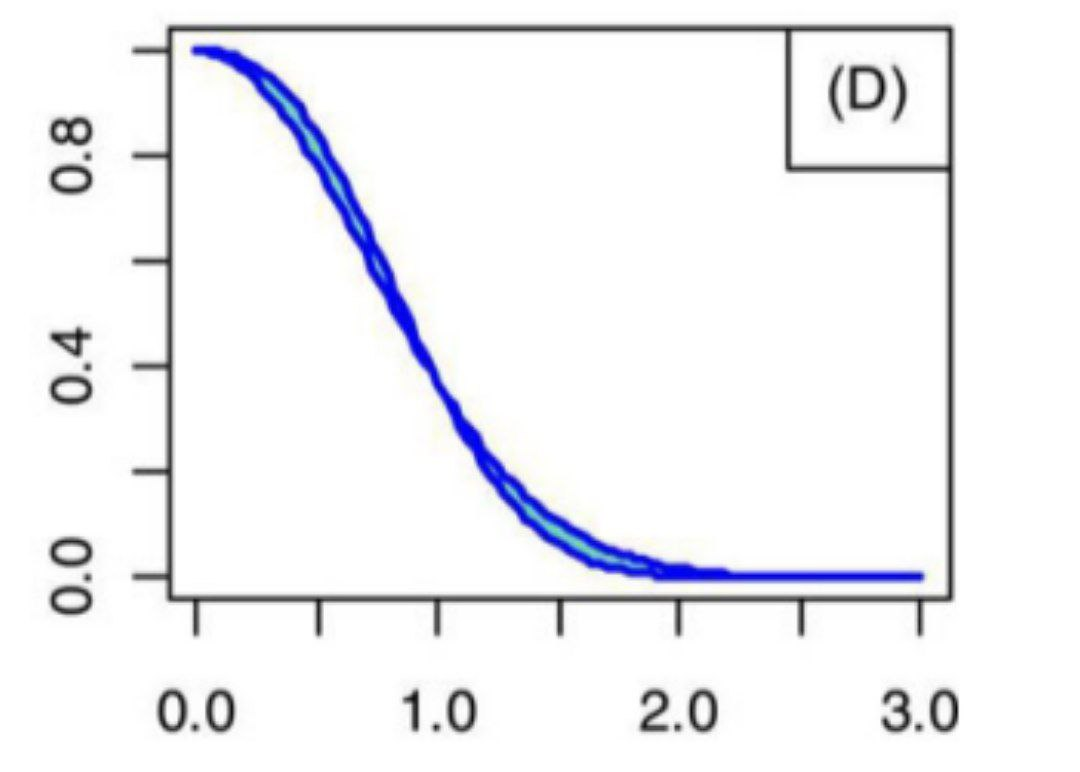
\includegraphics[width=0.35\linewidth]{h}}
\caption{survival function curve of neutrosophic weibull distribution with different shape parameters}
\end{figure}
\begin{center}
\hspace{2cm}
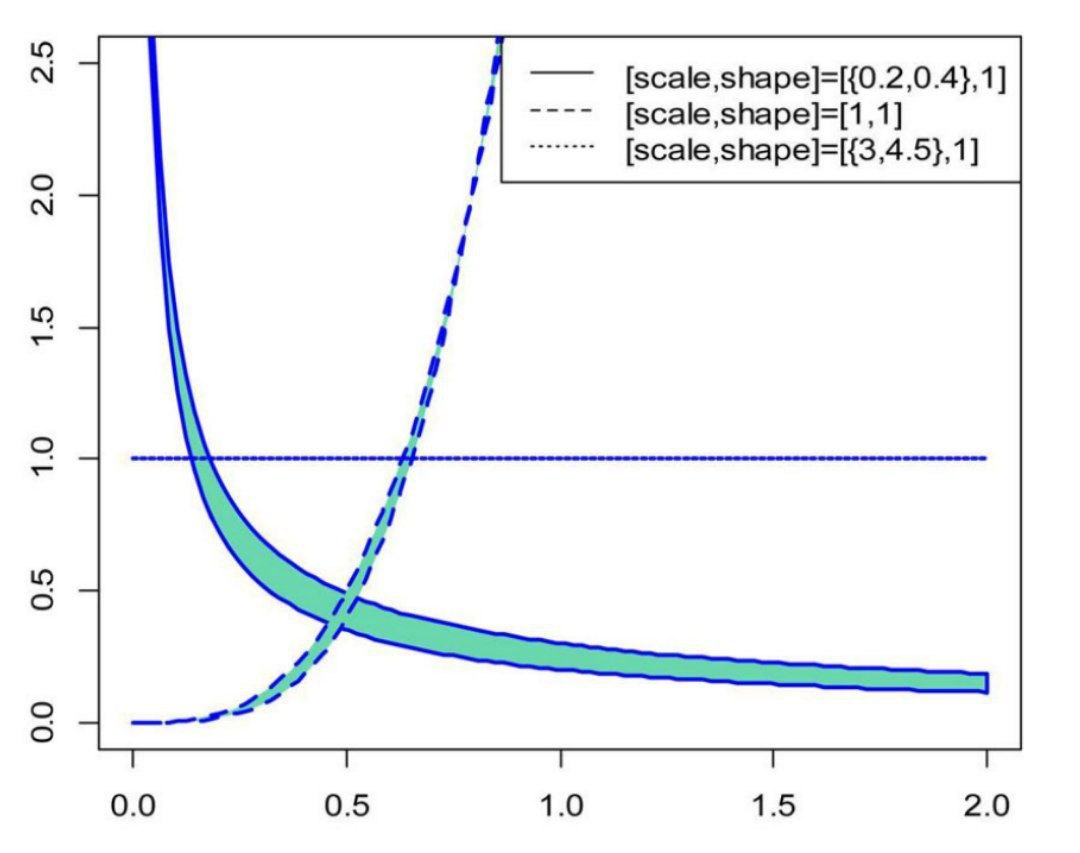
\includegraphics[width=0.7\textwidth]{hazard}
\newline 
Figure 4: hazard function of weibull distribution at various shape and scale parameters
\end{center}\newpage
\textrm{\textit{\textbf{\underline{Theoritcal derivations:$-$}}}}\newline\newline
The CDF of Neutrosophic Weibull Distribution is defined as,\\
 \begin{singlespace}
\hspace{5cm}$F_{N}$(x;${\lambda_{N}},k_{N})=\int_{0}^{x}f_{N}(t;{\lambda_{N}},k_{N})$dt
\end{singlespace}
which implies,
\begin{singlespace}
$F_{N}(x;{\lambda_{N}},k_{N})= \Biggl[\bigint_{0}^{x}$ $\dfrac{k_{l}}{{\lambda}_{l}}$ $\left(\dfrac{t}{\lambda_{l}}\right)^{k_{l}-1}$ $e^{-\left(\dfrac{t}{\lambda_{l}}\right)^{k_{l}}}$dt,$\bigint_{0}^{x}$ $\dfrac{k_{u}}{{\lambda}_{u}}$ $\left(\dfrac{t}{\lambda_{u}}\right)^{k_{u}-1}$ $e^{-\left(\dfrac{t}{\lambda_{u}}\right)^{k_{u}}}dt\Biggr]$
\end{singlespace}
Substituting $\left(\dfrac{t}{\lambda_{N}}\right)^{k_{N}}$ = p we get,
\begin{singlespace}
\hspace{5cm}$F_{N}(x;{\lambda_{N}},k_{N})= \Biggl[\bigint_{0}^{\left(\dfrac{x}{\lambda_{l}}\right)^{k_{l}}}$ $e^{-p}dp,\bigint_{0}^{\left(\dfrac{x}{\lambda_{u}}\right)^{k_{u}}}$ $e^{-p}dp\Biggr]$
\end{singlespace}\vspace{2cm}
which simplifies to,
\begin{singlespace}
\hspace{5cm}$F_{N}(x;{\lambda_{N}},k_{N})=\Biggl[1-e^{-\left(\dfrac{x}{\lambda_{l}}\right)^{k_{l}}},1-e^{-\left(\dfrac{x}{\lambda_{u}}\right)^{k_{u}}}\Biggr]$
\end{singlespace}
Which equals to,\\
\hspace*{5.5cm}$\boxed{F_{N}(x;{\lambda_{N}},k_{N})=1-e^{-\left(\dfrac{x}{\lambda_{N}}\right)^{k_{N}}}}$\newline\newline
By definition the survival function can be written in the form,\\
\begin{center}
$S_{N}(x)=1-F_{N}(x)$
\end{center}
So,it becomes,\\
\begin{center}
$1-\Biggl[1-e^{-\left(\dfrac{x}{\lambda_{N}}\right)^{k_{N}}}\Biggr]$
\end{center}
Which simplifies to,
\begin{center}
$\left[e^{-\left(\dfrac{x}{\lambda_{l}}\right)^{k_{l}}},e^{-\left(\dfrac{x}{\lambda_{u}}\right)^{k_{u}}}\right]$
\end{center}
\begin{center}
$\boxed{S_{N}(x)=e^{-\left(\dfrac{x}{\lambda_{N}}\right)^{k_{N}}}}$
\end{center}
\newpage
The hazard rate is given by,\\
\hspace*{5cm}$h_{N}(x)=\dfrac{f_{N}(x)}{S_{N}(x)}$\newline\newline\newline
\hspace*{5cm}=$\Biggl[\dfrac{\dfrac{k_{l}}{\lambda_{l}}\left(\dfrac{x}{\lambda_{l}}\right)^{k_{l}-1}e^{-\left(\dfrac{x}{\lambda_{l}}\right)^{k_{l}}}}{e^{-\left(\dfrac{x}{\lambda_{l}}\right)^{k_{l}}}},\dfrac{\dfrac{k_{u}}{\lambda_{u}}\left(\dfrac{x}{\lambda_{u}}\right)^{k_{u}-1}e^{-\left(\dfrac{x}{\lambda_{u}}\right)^{k_{u}}}}{e^{-\left(\dfrac{x}{\lambda_{u}}\right)^{k_{u}}}}\Biggr]$\newline\newline\newline
\hspace*{5cm}=$\Biggl[\dfrac{k_{l}}{\lambda_{l}}\left(\dfrac{x}{\lambda_{l}}\right)^{k_{l}-1},\dfrac{k_{u}}{\lambda_{u}}\left(\dfrac{x}{\lambda_{u}}\right)^{k_{u}-1}\Biggr]$\newline\newline
\hspace*{5cm}=$\boxed{\dfrac{k_{N}}{\lambda_{N}}\left(\dfrac{x}{\lambda_{N}}\right)^{k_{N}-1}}$
\begin{singlespace}
\vspace*{2cm} The Expectation of neutrosophic weibull distribution is given by,
\end{singlespace}
\begin{center}
\hspace{5cm}$E_{N}(X)=\bigint_{0}^{\infty}$ $xf_{N}$(x;${\lambda_{N}},k_{N})$dx\newline\newline
\begin{singlespace}
\hspace{5.5cm}=$\bigint_{0}^{\infty}$ $x\left(\dfrac{k_{N}}{{\lambda_{N}}}\right)$ $\left(\dfrac{x}{\lambda_{N}}\right)^{k_{N}-1}$ $e^{-\left(\dfrac{x}{\lambda_{N}}\right)^{k_{N}}}$dx
\end{singlespace}\vspace*{1cm}
\hspace{1cm}=$\Biggl[\bigint_{0}^{\infty}$ $x\left(\dfrac{k_{l}}{{\lambda_{l}}}\right)$ $\left(\dfrac{x}{\lambda_{l}}\right)^{k_{l}-1}$ $e^{-\left(\dfrac{x}{\lambda_{l}}\right)^{k_{l}}}$dx\hspace{2mm},\hspace{2mm} $\bigint_{0}^{\infty}$ $x\left(\dfrac{k_{u}}{{\lambda_{u}}}\right)$ $\left(\dfrac{x}{\lambda_{u}}\right)^{k_{u}-1}$ $e^{-\left(\dfrac{x}{\lambda_{u}}\right)^{k_{u}}}dx\Biggr]$
\end{center}
substituting $\left(\dfrac{x}{{\lambda_{N}}}\right)^{k_{N}}$=p we get,\\
\newline
\hspace{2cm}$\left(\dfrac{k}{\lambda_{N}}\right)\left(\dfrac{x}{{\lambda_{N}}}\right)^{k_{N}-1}$dx=dp\\
\newline so it simplifies to,
\begin{center}
E($X_{N}$)=$\Biggl[\dfrac{\lambda_{l}^{k_{l}+1}}{\lambda_{l}^{k_{l}}} \bigint_{0}^{\infty} p^{\dfrac{1}{k_{l}}+1-1}e^{-p}dp\hspace{2mm},\hspace{2mm}\dfrac{\lambda_{u}^{k_{u}+1}}{\lambda_{u}^{k_{u}}} \bigint_{0}^{\infty} p^{\dfrac{1}{k_{u}}+1-1}e^{-p}dp\Biggr]$
\end{center}
\begin{singlespace}
\hspace*{4.5cm}=$\Biggl[{\lambda_{l}}\Gamma\left(\dfrac{1}{k_{l}}+1\right)\hspace{2mm},\hspace{2mm}{\lambda_{u}}\Gamma\left(\dfrac{1}{k_{u}}+1\right)\Biggr]$
\end{singlespace}
\hspace*{4.5cm}=$\boxed{{\lambda_{N}}\Gamma\left(\dfrac{1}{k_{N}}+1\right)}$
\newline\newline
To get the variance in neutrosophic approach, we require the second order raw moment of neutrosophic Weibull distribution,\\
\begin{center}
E($X_{N}^{2}$)=$\bigint_{0}^{\infty}$ $x^{2}f_{N}$(x;${\lambda_{N}},k_{N})$dx\newline\newline
\begin{singlespace}
\hspace{1cm}=$\bigint_{0}^{\infty}$ $x^{2}\left(\dfrac{k_{N}}{{\lambda_{N}}}\right)$ $\left(\dfrac{x}{\lambda_{N}}\right)^{k_{N}-1}$ $e^{-\left(\dfrac{x}{\lambda_{N}}\right)^{k_{N}}}$dx
\end{singlespace}\vspace*{1cm}
=$\Biggl[\bigint_{0}^{\infty}$ $x^{2}\left(\dfrac{k_{l}}{{\lambda_{l}}}\right)$ $\left(\dfrac{x}{\lambda_{l}}\right)^{k_{l}-1}$ $e^{-\left(\dfrac{x}{\lambda_{l}}\right)^{k_{l}}}$dx\hspace{2mm},\hspace{2mm} $\bigint_{0}^{\infty}$ $x^{2}\left(\dfrac{k_{u}}{{\lambda_{u}}}\right)$ $\left(\dfrac{x}{\lambda_{u}}\right)^{k_{u}-1}$ $e^{-\left(\dfrac{x}{\lambda_{u}}\right)^{k_{u}}}dx\Biggr]$
\end{center}
substituting $\left(\dfrac{x}{{\lambda_{N}}}\right)^{k_{N}}=$p we get,\\
\newline
\hspace{2cm}$\left(\dfrac{k}{\lambda_{N}}\right)\left(\dfrac{x}{{\lambda_{N}}}\right)^{k_{N}-1}dx=dp$\\
\newline so it simplifies to,
\begin{center}
E($X_{N}^{2}$)=$\Biggl[\dfrac{\lambda_{l}^{k_{l}+2}}{\lambda_{l}^{k_{l}}} \bigint_{0}^{\infty} p^{\dfrac{2}{k_{l}}+1-1}e^{-p}dp\hspace{2mm},\hspace{2mm}\dfrac{\lambda_{u}^{k_{u}+2}}{\lambda_{u}^{k_{u}}} \bigint_{0}^{\infty} p^{\dfrac{2}{k_{u}}+1-1}e^{-p}dp\Biggr]$
\end{center}
\begin{singlespace}
\hspace*{4.5cm}=$\Biggl[{\lambda_{l}^{2}}\Gamma\left(\dfrac{2}{k_{l}}+1\right)\hspace{2mm},\hspace{2mm}{\lambda_{u}^{2}}\Gamma\left(\dfrac{2}{k_{u}}+1\right)\Biggr]$
\end{singlespace}
\hspace*{4.5cm}=$\boxed{{\lambda_{N}^{2}}\Gamma\left(\dfrac{2}{k_{N}}+1\right)}$
\newline\newline
So,the variance becomes,\\
\begin{center}
=$\Biggl[{\lambda_{l}^{2}}\Gamma\left(\dfrac{2}{k_{l}}+1\right)\hspace{2mm},\hspace{2mm}{\lambda_{u}^{2}}\Gamma\left(\dfrac{2}{k_{u}}+1\right)\Biggr]-\Biggl[{\lambda_{l}^{2}}\Gamma\left(\dfrac{1}{k_{l}}+1\right)^{2}\hspace{2mm},\hspace{2mm}{\lambda_{u}^{2}}\Gamma\left(\dfrac{1}{k_{u}}+1\right)^{2}\Biggr]$\newline\newline\newline
=$\Biggl[{\lambda_{l}^{2}}\Gamma\left(\dfrac{2}{k_{l}}+1\right)-{\lambda_{l}^{2}}\Gamma\left(\dfrac{1}{k_{l}}+1\right)^{2}\Biggr]\hspace{2mm},\hspace{2mm}\Biggl[{\lambda_{u}^{2}}\Gamma\left(\dfrac{2}{k_{u}}+1\right)-{\lambda_{u}^{2}}\Gamma\left(\dfrac{1}{k_{u}}+1\right)^{2}\Biggr]$\newline\newline\newline\newline Therefore,\hspace{2mm}
$\boxed{Var_{N}(x)=\Biggl[{\lambda_{N}^{2}}\left(\Gamma\left(\dfrac{2}{k_{N}}+1\right)-\Gamma\left(\dfrac{1}{k_{N}}+1\right)^{2}\right)\Biggr]}$
\end{center}
\newpage
The rth order raw moment for Neutrosophic Weibull Distribution  is defined as,
\begin{center}
E($X_{N}^{r}$)=$\bigint_{0}^{\infty}$ $x^{r}f_{N}$(x;${\lambda_{N}},k_{N})$dx\\
\begin{singlespace}
\hspace{4.3cm}=$\bigint_{0}^{\infty}$ $x^{r}\left(\dfrac{k_{N}}{{\lambda_{N}}}\right)$ $\left(\dfrac{x}{\lambda_{N}}\right)^{k_{N}-1}$ $e^{-\left(\dfrac{x}{\lambda_{N}}\right)^{k_{N}}}$dx
\end{singlespace}\vspace*{1cm}
=$\Biggl[\bigint_{0}^{\infty}$ $x^{r}\left(\dfrac{k_{l}}{{\lambda_{l}}}\right)$ $\left(\dfrac{x}{\lambda_{l}}\right)^{k_{l}-1}$ $e^{-\left(\dfrac{x}{\lambda_{l}}\right)^{k_{l}}}$dx\hspace{2mm},\hspace{2mm} $\bigint_{0}^{\infty}$ $x^{r}\left(\dfrac{k_{u}}{{\lambda_{u}}}\right)$ $\left(\dfrac{x}{\lambda_{u}}\right)^{k_{u}-1}$ $e^{-\left(\dfrac{x}{\lambda_{u}}\right)^{k_{u}}}dx\Biggr]$
\end{center}
substituting $\left(\dfrac{x}{{\lambda_{N}}}\right)^{k_{N}}$=p we get,\\
\newline
\hspace{2cm}$\left(\dfrac{k}{\lambda_{N}}\right)\left(\dfrac{x}{{\lambda_{N}}}\right)^{k_{N}-1}$dx=dp\\
\newline so it simplifies to,
\begin{center}
E($X_{N}^{r}$)=$\Biggl[\dfrac{\lambda_{l}^{k_{l}+r}}{\lambda_{l}^{k_{l}}} \bigint_{0}^{\infty} p^{\dfrac{r}{k_{l}}+1-1}e^{-p}dp\hspace{2mm},\hspace{2mm}\dfrac{\lambda_{u}^{k_{u}+r}}{\lambda_{u}^{k_{u}}} \bigint_{0}^{\infty} p^{\dfrac{r}{k_{u}}+1-1}e^{-p}dp\Biggr]$
\end{center}
\begin{singlespace}
\hspace*{4.5cm}=$\Biggl[{\lambda_{l}^{r}}\Gamma\left(\dfrac{r}{k_{l}}+1\right)\hspace{2mm},\hspace{2mm}{\lambda_{u}^{r}}\Gamma\left(\dfrac{r}{k_{u}}+1\right)\Biggr]$
\end{singlespace}
\hspace*{4.5cm}=$\boxed{{\lambda_{N}^{r}}\Gamma\left(\dfrac{r}{k_{N}}+1\right)}$\newline\newline
So,the mean can be obtained by putting r=1 in the above expression,\newline\newline
\hspace*{2cm} ${\mu}_{1N}={\mu}'_{1N}$=${\lambda_{N}}\Gamma\left(\dfrac{1}{k_{N}}+1\right)$\newline\newline
Similarly,\newline\newline
\hspace*{2cm} ${\mu}_{2N}={\mu}'_{2N}-{{\mu}'_{1N}}^{2}$=$\lambda_{N}^{2}\Biggl[\Gamma\left(\dfrac{2}{k_{N}}+1\right)-{\left(\Gamma\left(\dfrac{1}{k_{N}}+1\right)\right)^{2}}\Biggr]$\newline\newline
Now,\newline\newline
${\mu}_{3N}={\mu}'_{3N}-3{{\mu}'_{2N}}{{\mu}'_{1N}}+2({\mu}'_{1N})^{3}$=$\boxed{{\lambda_{N}}^{3}\Biggl[\Gamma\left(\dfrac{3}{k_{N}}+1\right)$ $-$ 3$\Gamma\left(\dfrac{1}{k_{N}}+1\right)$ $\Gamma\left(\dfrac{2}{k_{N}}+1\right)$ $+$2$\Gamma\left(\dfrac{1}{k_{N}}+1\right)^{3}\Biggr]}$\newline\newline
Again,\newline\newline
${\mu}_{4N}={\mu}'_{4N}-4{{\mu}'_{3N}}{{\mu}'_{1N}}+6{{\mu}'_{2N}}{{{\mu}'_{1N}}^{2}}-3{{{\mu}'_{1N}}^{4}}$\\
=\resizebox{1\hsize}{!}{$\boxed{{\lambda_{N}}^{4}\Biggl[\Gamma\left(\dfrac{4}{k_{N}}+1\right)-4\Gamma\left(\dfrac{3}{k_{N}}+1\right)\Gamma\left(\dfrac{1}{k_{N}}+1\right)+6\Gamma\left(\dfrac{2}{k_{N}}+1\right)\left(\Gamma\left(\dfrac{1}{k_{N}}+1\right)\right)^{2}-3\left(\Gamma\left(\dfrac{1}{k_{N}}+1\right)\right)^{4}\Biggr]}$}\newpage
The coefficient of skewness is defined as,\newline\newline
\hspace*{5cm}$Sk_{N}=\dfrac{{\mu}_{3N}}{\left(\mu_{2N}\right)^{\dfrac{3}{2}}}$
\begin{singlespace}
So,$Sk_{l}=\dfrac{\Biggl[\Gamma\left(\dfrac{3}{k_{l}}+1\right) - 3\Gamma\left(\dfrac{1}{k_{l}}+1\right) \Gamma\left(\dfrac{2}{k_{l}}+1\right) +2\Gamma\left(\dfrac{1}{k_{l}}+1\right)^{3}\Biggr]}{\Biggl[\Gamma\left(\dfrac{2}{k_{l}}+1\right)-{\left(\Gamma\left(\dfrac{1}{k_{l}}+1\right)\right)^{2}}\Biggr]^{\dfrac{3}{2}}}$
\end{singlespace}
\begin{singlespace}
So,$Sk_{u}=\dfrac{\Biggl[\Gamma\left(\dfrac{3}{k_{u}}+1\right) - 3\Gamma\left(\dfrac{1}{k_{u}}+1\right) \Gamma\left(\dfrac{2}{k_{u}}+1\right) +2\Gamma\left(\dfrac{1}{k_{u}}+1\right)^{3}\Biggr]}{\Biggl[\Gamma\left(\dfrac{2}{k_{u}}+1\right)-{\left(\Gamma\left(\dfrac{1}{k_{u}}+1\right)\right)^{2}}\Biggr]^{\dfrac{3}{2}}}$
\end{singlespace}
\vspace*{2cm}where,$\boxed{Sk_{N}=[Sk_{l},Sk_{u}]}$\newline\newline
The coefficient of kurtosis is given by,\\
\begin{center}
$\dfrac{{\mu}_{4N}}{{\mu}_{2N}^{2}}$
\end{center}
Which equals to,\\
$\dfrac{\Biggl[\Gamma\left(\dfrac{4}{k_{N}}+1\right)-4\Gamma\left(\dfrac{3}{k_{N}}+1\right)\Gamma\left(\dfrac{1}{k_{N}}+1\right)+6\Gamma\left(\dfrac{2}{k_{N}}+1\right)\left(\Gamma\left(\dfrac{1}{k_{N}}+1\right)\right)^{2}-3\left(\Gamma\left(\dfrac{1}{k_{N}}+1\right)\right)^{4}\Biggr]}{\Biggl[\Gamma\left(\dfrac{2}{k_{N}}+1\right)-{\left(\Gamma\left(\dfrac{1}{k_{N}}+1\right)\right)^{2}}\Biggr]^{2}}$\\
The coefficient of excess kurtosis is defined as,\\
\begin{center}
$\dfrac{{\mu}_{4N}}{{\mu}_{2N}^{2}}-3$
\end{center}
After simplifying it becomes,\\
\resizebox{1\hsize}{!}{$\boxed{\dfrac{\Biggl[-6\left(\Gamma\left(\dfrac{1}{k_{N}}+1\right)\right)^{4}+12\Gamma\left(\dfrac{2}{k_{N}}+1\right)\left(\Gamma\left(\dfrac{1}{k_{N}}+1\right)\right)^{2}-4\Gamma\left(\dfrac{3}{k_{N}}+1\right)\Gamma\left(\dfrac{1}{k_{N}}+1\right)+\Gamma\left(\dfrac{4}{k_{N}}+1\right)-3{\Gamma\left(\dfrac{2}{k_{N}}+1\right)^{2}}\Biggr]}{\Biggl[\Gamma\left(\dfrac{2}{k_{N}}+1\right)-{\left(\Gamma\left(\dfrac{1}{k_{N}}+1\right)\right)^{2}}\Biggr]^{2}}}$}\\
\newpage
The median of NWD can be calculated by solving,\newline\newline\newline
\hspace*{5cm}$F_{N}(\xi_{med})=\dfrac{1}{2}$\newline\newline\newline
\hspace*{4cm}$\implies 1-e^{-\left(\dfrac{\xi_{med}}{\lambda_{N}}\right)^{k_{N}}}=\dfrac{1}{2}$\newline\newline\newline
\hspace*{4cm}$\implies e^{-\left(\dfrac{\xi_{med}}{\lambda_{N}}\right)^{k_{N}}}=\dfrac{1}{2}$\newline\newline
which simplifies to,\\
\hspace*{5cm}$\boxed{\xi_{med}=\lambda_{N}[ln2]^{\dfrac{1}{k_{N}}}}$\newline\newline\newline
\textrm{\textit{\textbf{\underline{Maximum Likelihood Estimation:$-$}}}}\newline\newline
To, estimate the neutrosophic parameters of NWD we use MLE approach.In MLE approach we take independent observation from the same distribution and based on that we estimate our parameters.As,we take sample from same distribution they became identical too.In this method we form the likelihood function based on those samples and then find the value of the parameters which maximizes the likelihood function.MLE is often considered because of it's minimum variance and asymptotic unbiasedness property.Let $x_{1},x_{2},...,x{n}$ be n i.i.d survival times which follows NWD.So, the joint density is given by,\newline\newline\newline
\hspace*{5cm}$\mathscr{L}(\vec{x}|\lambda_{N},k_{N})=\prod_{i=1}^{n}f(x_{i}|\lambda_{N},k_{N})$\newline\newline
\hspace*{5cm}=$\prod_{i=1}^{n}\Biggl[\dfrac{k_{N}}{\lambda_{N}}\left(\dfrac{x_{i}}{\lambda_{N}}\right)^{k_{N}-1}e^{-\left(\dfrac{x_{i}}{\lambda_{N}}\right)^{k_{N}}}\Biggr]$\newline\newline
\hspace*{5cm}=$\Biggl[\dfrac{k_{N}^{n}}{\lambda_{N}^{n}}\prod_{i=1}^{n}x_{i}^{k_{N}-1}e^{-\left(\dfrac{x_{i}}{\lambda_{N}}\right)^{k_{N}}}\Biggr]$\\
Taking logarithm on both sides we get,\\
$ln(\mathscr{L}(\vec{x}|\lambda_{N},k_{N}))=nln(k_{N})-nln(\lambda_{N})+(k_{N}-1)\sum_{i=1}^{n}ln(x_{i})-{\sum_{i=1}^{n}\left(\dfrac{x_{i}}{\lambda_{N}}\right)^{k_{N}}}$\newline\newline\newline
Now partially differentiating and equating them with 0 gives,\newline\newline\newline
\hspace*{4cm}$\Biggl[\dfrac{\delta(ln(\mathscr{L}(\vec{x}|\lambda_{N},k_{N})))}{\delta\lambda_{N}},\dfrac{\delta(ln(\mathscr{L}(\vec{x}|\lambda_{N},k_{N})))}{\delta k_{N}}\Biggr]=\Biggl[0,0\Biggr]$\newline\newline\newline\newline
So,we can write them as,\newline\newline\newline
\begin{math}
\begin{array}{l}
\Biggl[\dfrac{\delta(ln(\mathscr{L}(\vec{x}|\lambda_{N},k_{N})))}{\delta\lambda_{l}},\dfrac{\delta(ln(\mathscr{L}(\vec{x}|\lambda_{N},k_{N})))}{\delta\lambda_{u}}\Biggr]=[0,0]\\
\newline\newline\newline
\Biggl[\dfrac{\delta(ln(\mathscr{L}(\vec{x}|\lambda_{N},k_{N})))}{\delta k_{l}},\dfrac{\delta(ln(\mathscr{L}(\vec{x}|\lambda_{N},k_{N})))}{\delta k_{u}}\Biggr]=[0,0]
\end{array}
\Biggr\}
\end{math}
$..............(1)$
\newline\newline\newline
So,these equations has no closed form we need to use numerical iterative techniques such as Newton-Raphson method or scoring methods to find the estimated parameters.\newpage
\textrm{\textit{\textbf{\underline{Simulation of Neutrosophic Weibull Distribution and Estimation of parameters:$-$}}}}\newline\newline
To, simulate data from neutrosophic weibull distribution we need the method of Monte Carlo Estimation.This approach enables  us to generate computer based pseudo random number generator for generating random numbers.Here, we use the library package "ntsDists" in R to generate  neutrosophic random numbers from weibull distribution and estimate the parameters using newton raphson iterative technique.\newline\newline
Here, we have generated 10000 samples from neutrosophic weibull distribution with scale parameter [9.5544,10.3370] and shape parameter  the generated samples are,\newline\newline
$[1.669639e+01\hspace{1mm},\hspace{1mm}1.803153e+01]\hspace{1mm},\hspace{1mm}[1.186682e+01\hspace{1mm},\hspace{1mm}1.282987e+01]\hspace{1mm},\hspace{1mm[1.0519,1.0553]}[5.227939e+00\hspace{1mm},\hspace{1mm}5.667158e+00]\hspace{1mm},\hspace{1mm}[2.967674e+01\hspace{1mm},\hspace{1mm}3.199053e+01]\hspace{1mm},\hspace{1mm}[7.889716e+00\hspace{1mm},\hspace{1mm}8.541229e+00]\hspace{1mm},\hspace{1mm}[5.348771e+00\hspace{1mm},\hspace{1mm}5.797715e+00]\hspace{1mm},\hspace{1mm}[5.213533e+00\hspace{1mm},\hspace{1mm}5.651591e+00]\hspace{1mm},\hspace{1mm}[1.073665e+01\hspace{1mm},\hspace{1mm}1.161173e+01]\hspace{1mm},\hspace{1mm}[1.202369e+01\hspace{1mm},\hspace{1mm}1.299892e+01]\hspace{1mm},\hspace{1mm}[2.685068e-01,2.938626e-01]..........$\newline\newline
The density plot of the generated neutrosophic weibull distribution looks like,\\
\begin{center}
\hspace{2cm}
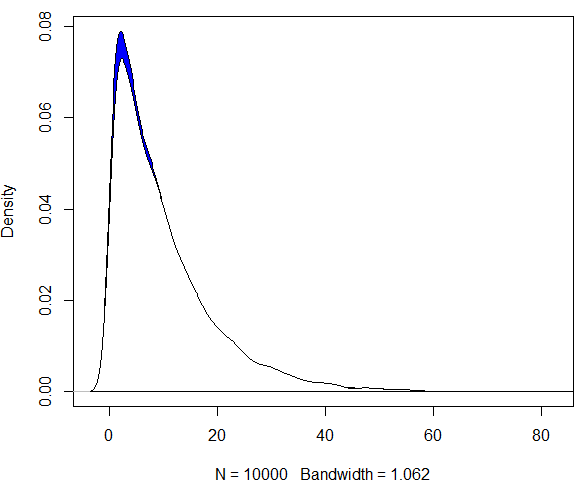
\includegraphics[width=0.7\textwidth]{nwd}
\newline 
Figure 1: Neutrosophic Weibull pdf for various values of the shape and scale parameter 
\end{center}
\begin{center}
\hspace{2cm}
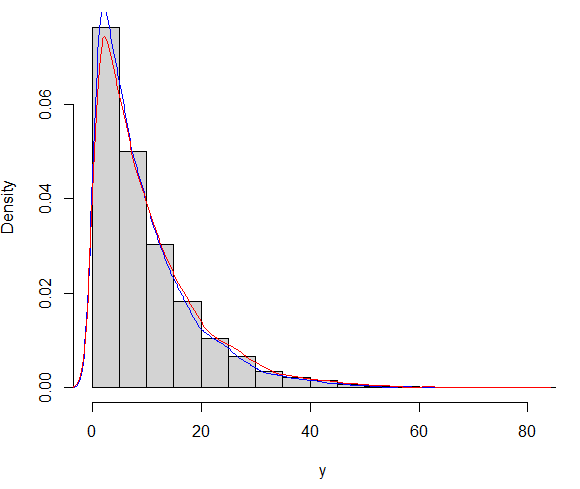
\includegraphics[width=0.7\textwidth]{hcwd}
\newline 
Figure 2: Histogram of Neutrosophic Weibull for various values of the shape and scale parameter 
\end{center}
\begin{center}
\hspace{2cm}
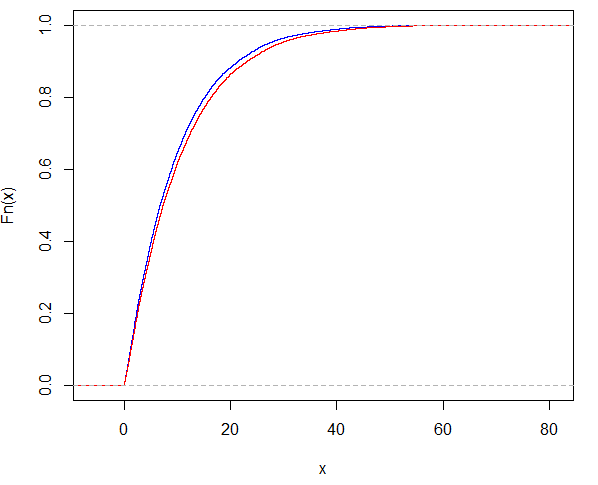
\includegraphics[width=0.7\textwidth]{cnwd}
\newline 
Figure 3: Neutrosophic Weibull cdf for various values of the shape and scale parameter 
\end{center}
The maximum likelihood estimation for the parameters gives us the value as,\\
\begin{singlespace}
\hspace{5cm} MLE(shape parameter)($\hat{k}$)= $\boxed{[1.062414\hspace{1mm},\hspace{1mm}1.054294]}$\\
\hspace*{5.6cm} MLE(scale parameter)($\hat{\lambda}$)=$\boxed{[ 9.687938\hspace{1mm},\hspace{1mm}10.352736]}$
\end{singlespace}\newpage
So,the mean failure time based on estimated parameters is=${\hat{\lambda}_{N}}\Gamma\left(\dfrac{1}{\hat{k}_{N}}+1\right)$\\Which is equal to,\newline\newline
\hspace*{5cm}=$\Biggl[{\hat{\lambda}_{l}}\Gamma\left(\dfrac{1}{\hat{k}_{l}}+1\right)\hspace{1mm},\hspace{1mm}{\hat{\lambda}_{l}}\Gamma\left(\dfrac{1}{\hat{k}_{l}}+1\right)\Biggr]$\newline\newline
\hspace*{5cm}=$\boxed{\Biggl[9.460933\hspace{1mm},\hspace{1mm}10.13853\Biggr]}$\newline\newline
The sample mean is $=\boxed{[9.270696\hspace{1mm},\hspace{1mm}10.01847]}$\newline\newline\newline
The variance based on MLE estimates is=$\Biggl[{\hat{\lambda}_{N}^{2}}\left(\Gamma\left(\dfrac{2}{\hat{k}_{N}}+1\right)-\Gamma\left(\dfrac{1}{\hat{k}_{N}}+1\right)^{2}\right)\Biggr]$\newline\newline
\hspace*{2cm}$\Biggl[\biggl[{\hat{\lambda}_{l}^{2}}\Gamma\left(\dfrac{2}{\hat{k}_{l}}+1\right)-{\hat{\lambda}_{l}^{2}}\Gamma\left(\dfrac{1}{\hat{k}_{l}}+1\right)^{2}\biggr]\hspace{2mm},\hspace{2mm}\biggl[{\hat{\lambda}_{u}^{2}}\Gamma\left(\dfrac{2}{\lambda{k}_{u}}+1\right)-{\hat{\lambda}_{u}^{2}}\Gamma\left(\dfrac{1}{\hat{k}_{u}}+1\right)^{2}\biggr]\Biggr]$\newline\newline
Which is equal to,\newline\newline
\hspace*{5cm}=$\boxed{[79.38225\hspace{1mm},\hspace{1mm}92.5476]}$\newline\newline
The sample variance is equal to=$\boxed{[77.19573\hspace{1mm},\hspace{1mm}89.58036]}$\newline\newline
So,we represent the results of the analysis in the table below,\newline\newline
\begin{tabular}{ |p{5cm}|p{5cm}|p{5cm}|  }
\hline
\multicolumn{3}{|c|}{Estimated vs Observed Comparison} \\
\hline
Descriptive Measures & Observed Values & Estimated Values \\
\hline
Scale parameter & [9.5544,10.3370] & [ 9.687938,10.352736] \\
\hline
Shape parameter & [1.0519,1.0553] & [1.062414,1.054294] \\
\hline
mean& [9.270696,10.01847]  & [9.460933,10.13853] \\
\hline
median &[6.743455,7.304005] &[6.861323,7.3127]\\
\hline
variance   & [77.19573,89.58036] & [79.38225,92.5476] \\
\hline
skewness   & [1.854021,1.845088]&[1.860548,1.851586]\\
\hline
kurtosis   & [2.067178,2.012699] &[1.90106, 2.028742]\\
\hline
\end{tabular}
\vspace*{2cm}
\begin{singlespace}
\begin{Large}
\textrm{\textit{\textbf{\underline{Conclusions:$-$}}}}
\end{Large}
\end{singlespace}
Here,We discussed about the Neutrosophic Extension of Weibull distribution in Reliability analysis.At first, we develop the theortical derivations such as mean,variance,skewness,kurtosis of the proposed model and then we perform simulation by generating data from Neutrosophic weibull distribution using monte carlo simulation with the help of R software and validate the proposed model by fitting the data by comparing the observed descriptive measures and estimated descriptive measures using the estimated parameters which we got from MLE method.
\newpage
\begin{thebibliography}{11}
[1]\hspace{0.3cm}@book{texbook,
  author = {Florentin Smarandache ,Mohamed Abdel-Basset },
  title = {Neutrosophic Operational Research Methods and application},
  publisher = {springer}
}
\newline\newline
[2]\hspace{0.3cm}@article{research article,
  title={Neutrosophic Weibull distribution and Neutrosophic Family  
Weibull Distribution },
  author={Kawther Fawzi Hamza Alhasan and Florentin Smarandache},
  journal={UNM},
  year={2019},
  publisher={University of New Mexico}
}
\newline\newline
[3]\hspace{0.3cm}@article{research article,
  title={Neutrosophic Exponential Distribution: Modeling and Applications for Complex Data Analysis},
  author={Wen-Qi Duan,Zahid Khan
,Muhammad Gulistan
,and Adnan Khurshid},
  journal={Hindawi},
  year={2017},
  publisher={John Wiley and Sons,Inc.}
}
\newline\newline
[4]\hspace{0.3cm}@article{research article,
  title={.Neutrosophic Extension of the Maxwell Model: Properties and Applications},
  author={Faisal Shah,Muhammad Aslam,Zahid Khan
,Mohammed M. A. Almazah
,and Fuad S. Alduais},
  journal={Hindawi},
  year={2022},
  publisher={John Wiley and Sons,Inc.}
}
\newline\newline
[5]\hspace{0.3cm}@article{research article,
  title={Novel Open Source Python Neutrosophic Package },
  author={Haitham A. El-Ghareeb},
  journal={UNM},
  year={2019},
  publisher={University of New Mexico}
}
\newline\newline
[6]\hspace{0.3cm}@article{research article,
  title={Neutrosophic Generalized Exponential Distribution with Application },
  author={Gadde Srinivasa Rao,Mina Norouzirad,Danial Mazarei},
  journal={UNM},
  year={2023},
  publisher={University of New Mexico}
}
\newline\newline
[7]\hspace{0.3cm}@book{texbook,
  author = {Florentin Smarandache},
  title = {Neutrosophic Theory and It's Application},
  publisher = {EuropaNova}
}
\newline\newline
[8]\hspace{0.3cm}@book{texbook,
  author = {Florentin Smarandache},
  title = {Introduction to Neutrosophic Statistics},
  publisher = {Sitech and Education Publishing}
}
\newline\newline
[9]\hspace{0.3cm}@book{texbook,
  author = {Florentin Smarandache,Yanhui Guo},
  title = {New Development of Neutrosophic Probability,Neutrosophic Statistics,Neutrosophic Algebric Structures,and Neutrosophic and Plithogenic Optimizations},
  publisher = {MDPI}
}
\newline\newline
[10]\hspace{0.3cm}https://cran.r-project.org/web/packages/ntsDists/ntsDists.pdf
\end{thebibliography}

\newpage
\begin{Large}
\textrm{\textit{\textbf{\underline{Appendix:$-$}}}}
\end{Large}
\newline\newline
R code to generate neutrosphic weibull distribution,\newline\newline
\begin{lstlisting}[language=R]
> library(ntsDists)

###Generating 10000 samples from Neutrosophic Weibull Distribution

>y=rnsweibull(n=10000,scale=c(9.5544,10.3370),shape=c(1.0519,1.0553))

###  The density curve of neutrosophic weibull distribution

> plot.new()
> plot(density(y[,1]),col="Blue")
> polygon(density(y[,1]),col="Blue")
> polygon(density(y[,2]),col="white") 

###  The histogram plot of neutrosophic weibull distribution

>plot.new()
>hist(y,freq = FALSE)
>lines(density(y[,1]),col="Blue")
>lines(density(y[,2]),col="red")

###  The cdf plot of neutrosophic weibull distribution

>plot.new()
>plot(ecdf(y[,1]),col="Blue")
>lines(ecdf(y[,2]),col="red")

### measures based on sample

>mean(y[,1])
>mean(y[,2])
>var(y[,1])
>var(y[,2])

### MLE estimates

>install.packages("EnvStats")
>library(EnvStats)
>eweibull(y[,1],method = "mle")
>eweibull(y[,2],method = "mle")

###MLE estimates without using package

>data <- rweibull(10000, shape =shape parameter, scale = scale parameter)
>data

>likelihood <- function(params, data) {
  scale <- params[1]
  shape <- params[2]
  -sum(dweibull(data, shape = shape, scale = scale, log = TRUE))
}       # Define the likelihood function for Weibull distribution

>mle_result <- optim(c(2, 5), likelihood, data = data, method = "L-BFGS-B")          # Use optim function to obtain MLE of parameters

>mle_scale <- mle_result$par[1]
>mle_shape <- mle_result$par[2]    # Extract MLE estimates

>cat("MLE of shape parameter:", mle_shape, "\n")
>cat("MLE of scale parameter:", mle_scale, "\n")    # Print MLE estimates

###Comparing observed and esimated descriptive measures

# Mean of Weibull distribution
>mean_failure_time <- gamma(1+1/mle_shape)*mle_scale 

# Calculate mean failure time and compare with sample mean
>sample_mean <- mean(data)    

>cat("Mean failure time (MLE):", mean_failure_time, "\n")
>cat("Sample mean:", sample_mean, "\n")     # Print mean values
\end{lstlisting}
\vspace*{3cm}
The python codes which can also be used,
\begin{lstlisting}[language=Python]
###Generate samples for neutrosophic weibull distribution

import numpy as np
import matplotlib.pyplot as plt

def weibull_pdf(x, shape, scale):
    return (shape / scale) * (x / scale)**(shape - 1) * 
    np.exp(-(x / scale)**shape)

def bounding_pdf(x, c):
    return c * np.exp(-c * x)

def acceptance_rejection(shape, scale, n_samples):
    max_pdf_ratio = weibull_pdf(scale, shape, scale) /
     bounding_pdf(scale, shape)
    samples = []
    while len(samples) < n_samples:
        x = np.random.exponential(scale=1/shape)  
        # Exponential distribution as a candidate
        u = np.random.uniform(0, max_pdf_ratio * bounding_pdf(x, shape))
        if u <= weibull_pdf(x, shape, scale):
            samples.append(x)
    return samples

# Parameters for the Weibull distribution
shape = shape parameter
scale = scale parameter

# Number of samples to generate
n_samples = 1000

# Generate samples using acceptance-rejection method
samples = acceptance_rejection(shape, scale, n_samples)

# Plot histogram of generated samples
plt.hist(samples, bins=30, density=True, alpha=0.7, color='blue',
 label='Generated samples')
# Plot the theoretical PDF
x_values = np.linspace(0, max(samples), 1000)
plt.plot(x_values, weibull_pdf(x_values, shape, scale), color='red',
 linewidth=2, label='Theoretical PDF')
plt.xlabel('x')
plt.ylabel('Probability Density')
plt.title('Samples from Weibull distribution (shape={}, scale={})'
.format(shape, scale))
plt.legend()
plt.show()




####Plot of pdf of neutrosophic weibull distribution

import seaborn as sns
sns.kdeplot(samples, color='blue', label='Sample 1', linestyle='-',
 linewidth=2,shade=1)
sns.kdeplot(samples1, color='red', label='Sample 2', linestyle='--',
 linewidth=2,shade=1)

# Add labels and title
plt.xlabel('X')
plt.ylabel('Density')
plt.title('Kernel Density Estimate (KDE) Plot of Two Different Samples')
plt.legend()

# Show plot
plt.show()
\end{lstlisting}
\end{document}